% -*- program:xelatex -*-

\documentclass[12pt]{beamer}

\usetheme{m}

\usepackage{booktabs}
\usepackage{multirow}
\usepackage{multicol}
\usepackage{minted}
\usepackage{hyperref}

\title{Teaching 
\includegraphics[width=0.3in]{imgs/R.png}$\,$ using the 
\includegraphics[width=0.7in]{imgs/github.png}$\,$ ecosystem}
\subtitle{}
\date{UseR! 2015 - Aalborg}
\author{Colin Rundel}
\institute{Duke University\\Department of Statistical Science}
% \titlegraphic{\hfill\includegraphics[height=1.5cm]{logo/logo}}

\begin{document}

\maketitle


\begin{frame}
\frametitle{Sta 523 - Statistical Programming}

Course details:
\begin{itemize}
\item First offered in Fall 2014
\item Core course in Masters of Statistical Science Program
\item Approximately 30 Students
\begin{itemize}
\item 2/3 MSS \& MSEM, 1/3 other MS \& PhD
\item Divided into teams of 3-4
\item Disparate backgrounds
\end{itemize}
\item Biweekly team programming assignments
\item Team final project, individual final exam
\end{itemize}

\end{frame}


\begin{frame}
\frametitle{Technical Learning Objectives}

\hspace{0.1in}

\includegraphics[width=0.95in]{imgs/R.png}
\hfill

\includegraphics[width=0.8in]{imgs/term.png}
\hfill

\includegraphics[width=0.8in]{imgs/git.jpg}
\hspace{0.1in}

\end{frame}

\begin{frame}
\frametitle{Methodological Learning Objectives}

Collaboration

\vspace{3mm}

Reproducible Research
\begin{itemize}
\item R Markdown / knitr
\item GNU Make
\end{itemize}

\vspace{3mm}

Data in the Real World
\begin{itemize}
\item Messy data
\item Non-flat data
\end{itemize}



\end{frame}


\begin{frame}
\frametitle{Infrastructure}

\vspace{-5mm}

Dedicated departmental server
\begin{itemize}
\item RStudio Server Pro
\item Individual departmental accounts
\item System wide install of core packages
\end{itemize}

\vspace{3mm}

Github Organization
\begin{itemize}
\item 1 private repo / team (Github Education)
\item Shared public repos (e.g. examples)
\end{itemize}

\vspace{3mm}

Continuous Integration
\begin{itemize}
\item TravisCI, Wercker, Drone, etc.
\end{itemize}

\end{frame}


\begin{frame}
\frametitle{Assignments}

All assignments are turned in via github (pull the repo at the deadline)

\vspace{3mm}

What do we get from this?
\begin{itemize}
\item Forces students to use version control
\item Simplifies course administration
\begin{itemize}
\item Code / documentation / scaffolding all in the same place
\item Easy to grab files (pull)
\item Easy to distribute files (push)
\end{itemize}
\item Searchability
\item Accountability
\end{itemize}

\end{frame}



\begin{frame}
\frametitle{Feedback}

\vspace{-7mm}

Grading and feedback is given via pull requests

\begin{center}
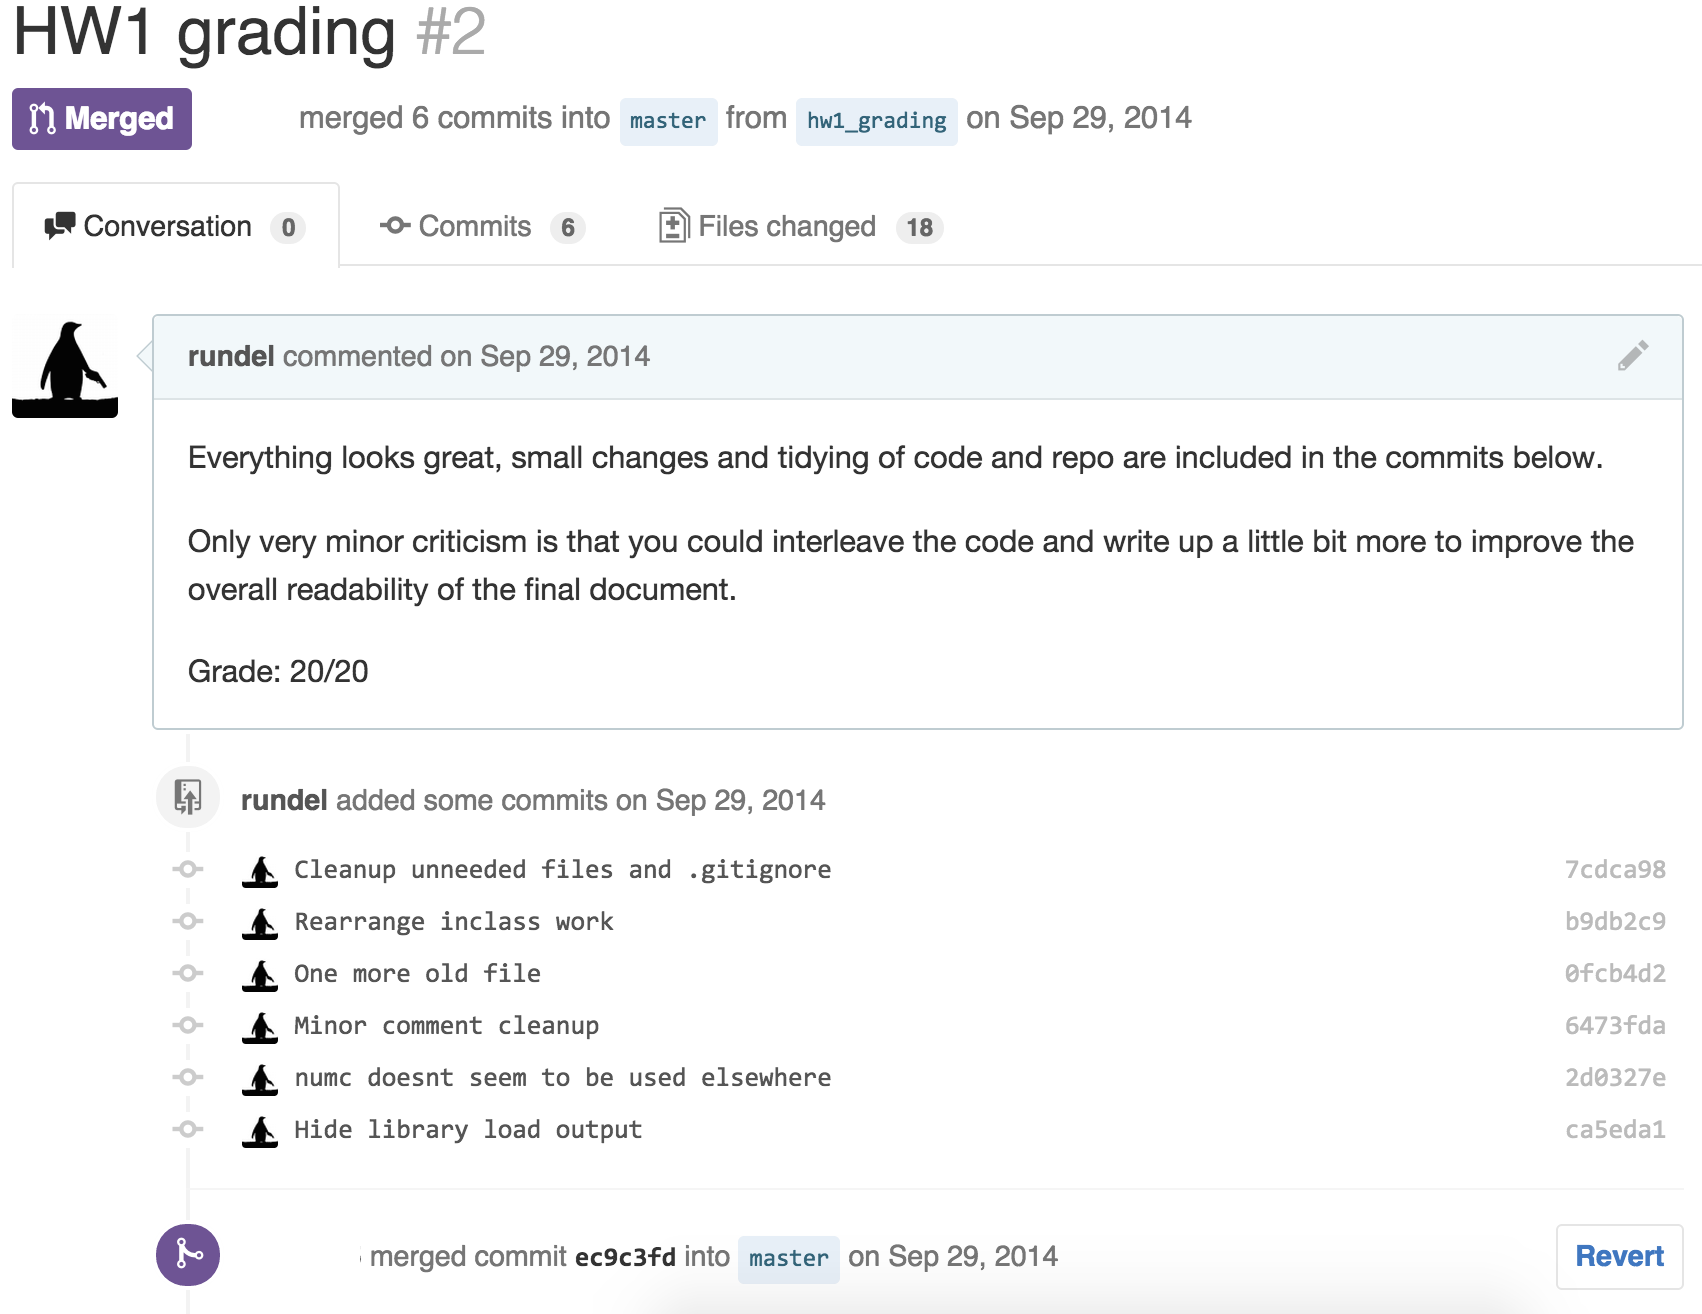
\includegraphics[width=0.8\textwidth]{imgs/github_pull_request.png}
\end{center}

\end{frame}



\begin{frame}
\frametitle{Course Process Cartoon}

\vspace{-7mm}

\begin{center}
\only<1-2>{
\includegraphics[width=0.5\textwidth]{imgs/cycle.png}}
\only<3>{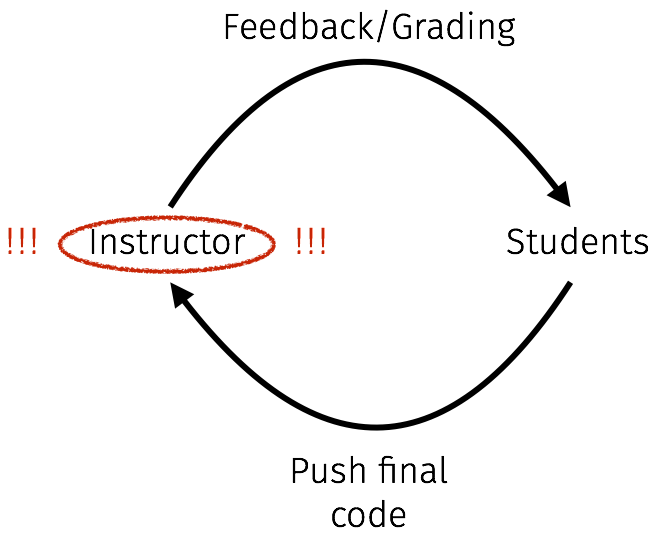
\includegraphics[width=0.5\textwidth]{imgs/cycle_ex.png}}
\end{center}

\pause

Github does improve both parts of this cycle \pause but doesn't address the fact that \emph{the instructor / TAs are the rate limiting step} (we don't scale well).

\end{frame}


\begin{frame}[fragile]
\frametitle{A painfully common conversation}

\vspace{-7mm}

{\footnotesize
\textit{Student: We've submitted our HW3!}
%
\begin{center} +1 Day \end{center}
%
\textit{Me: Your Rmd file doesn't knit, you used \mintinline{r}{setwd} with an absolute path.}
%
\begin{center} +1 Day \end{center}
%
\textit{Student: Ok we fixed that, does it work now?}
%
\begin{center} +1 Day \end{center}
%
\textit{Me: Nope, you used \mintinline{r}{lme4} without checking if it was installed.}
%
\begin{center} +1 Day \end{center}
%
\begin{center} $\vdots$ \end{center}
}
\end{frame}


\begin{frame}[fragile]
\frametitle{A solution?}

In the limited universe of this class,

\begin{align*}
\text{Me} &= \text{CRAN} \\
\\
\text{Student} &= \text{Package Developer}
\end{align*}

so what we want is some variant of \mintinline{shell}{R CMD check}.

\end{frame}


\begin{frame}
\frametitle{Check Features}

What should our \mintinline{shell}{R CMD check} look like?

\vspace{3mm}\pause

Ideally it should check that $\ldots$
\begin{itemize}
\item the code runs, Rmds knit
\item the coding style is consistent
\item the repo is tidy
\item the code runs in a reasonable time frame
\item the implementations are correct
\end{itemize}

\end{frame}


\begin{frame}
\frametitle{Automation}

\vspace{-5mm}

We would also like this to be done automatically.

\vspace{3mm}\pause

Again we can take a lesson from the package developers.

\vspace{3mm}

\begin{columns}
\column{0.9\textwidth}
\begin{center}
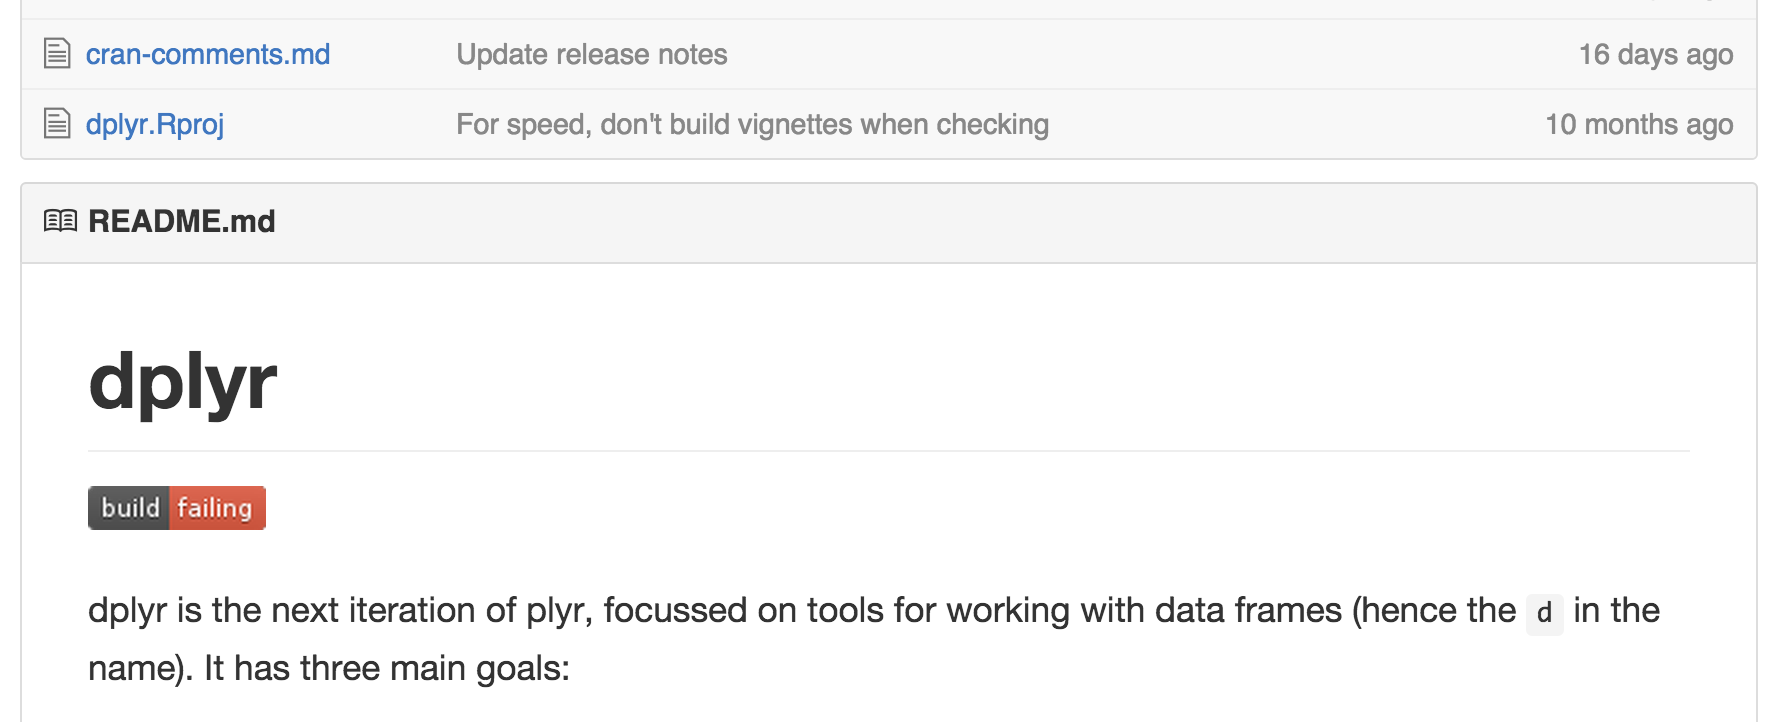
\includegraphics[width=0.9\textwidth]{imgs/dplyr_CI.png}
\end{center}

\column{0.1\textwidth}

\begin{center}

\includegraphics[width=0.3in]{imgs/travis.png}\\

\includegraphics[width=0.3in]{imgs/wercker.png}\\

\includegraphics[width=0.3in]{imgs/drone.png}\\

\includegraphics[width=0.3in]{imgs/jenkins.png}
\end{center}
\end{columns}

\end{frame}


\begin{frame}
\frametitle{Course Process Cartoon - Improved}

\vspace{-7mm}

\begin{center}
\only<1>{
\includegraphics[width=\textwidth]{imgs/cycle_ci.png}}
\only<2>{
\includegraphics[width=\textwidth]{imgs/cycle_ci_meme.png}}
\end{center}

\end{frame}


\begin{frame}[fragile]
\frametitle{Implementation}

This is currently more aspirational than reality, but the following is planned for the coming Fall 2015 semester.

\vspace{3mm}

Key details (subject to change):

\begin{itemize}
\item Adopting wercker for CI (uses Docker, \href{https://app.wercker.com/#buildstep/55883b8aade909cb4a0014b7}{steps})
\item Enforced coding style via \mintinline{r}{lintr}
\item Enforced directory structure
\item Allowed file/filetype whitelist
\item \mintinline{r}{testthat} for testing implementation assignments
\item automated scoring of prediction contests
\end{itemize}

\end{frame}


\begin{frame}
\frametitle{Conclusions}

Using github gives you a lot (for free) $\ldots$
\begin{multicols}{2}
\begin{itemize}
\item Version control
\item Accessible web UI
\item Education support
\item Collaboration tools
\item Search tools
\item CI tools
\end{itemize}
\end{multicols}

\vspace{3mm}

Needs of an R programming class are very similar to the needs of the R development community
\begin{itemize}
\item No need to reinvent the wheel - use the existing solutions
\item Teach the tools students will continue to use
\end{itemize}

\end{frame}



\begin{frame}[t]
\frametitle{Questions, Comments?}

\vspace{-6mm}

\begin{center}
{\small
\renewcommand*\arraystretch{2.5}
\begin{tabular}{ll}
\raisebox{-0.3\height}{
\includegraphics[width=0.3in]{imgs/email_icon.png}}  & rundel@gmail.com \\
\raisebox{-0.3\height}{
\includegraphics[width=0.3in]{imgs/github_icon.png}} & github.com/rundel/ \\
\raisebox{-0.3\height}{
\includegraphics[width=0.3in]{imgs/pres_icon.png}}   & github.com/rundel/Presentations/ \\
\raisebox{-0.3\height}{
\includegraphics[width=0.3in]{imgs/home_icon.png}}   & bit.ly/Sta523\_2014 {\large|} bit.ly/Sta523\_2015\\
\end{tabular}
}
\end{center}

\end{frame}



\end{document}
